\documentclass{standalone}
\usepackage{pgfplots}
\pgfplotsset{compat=newest}

\begin{document}
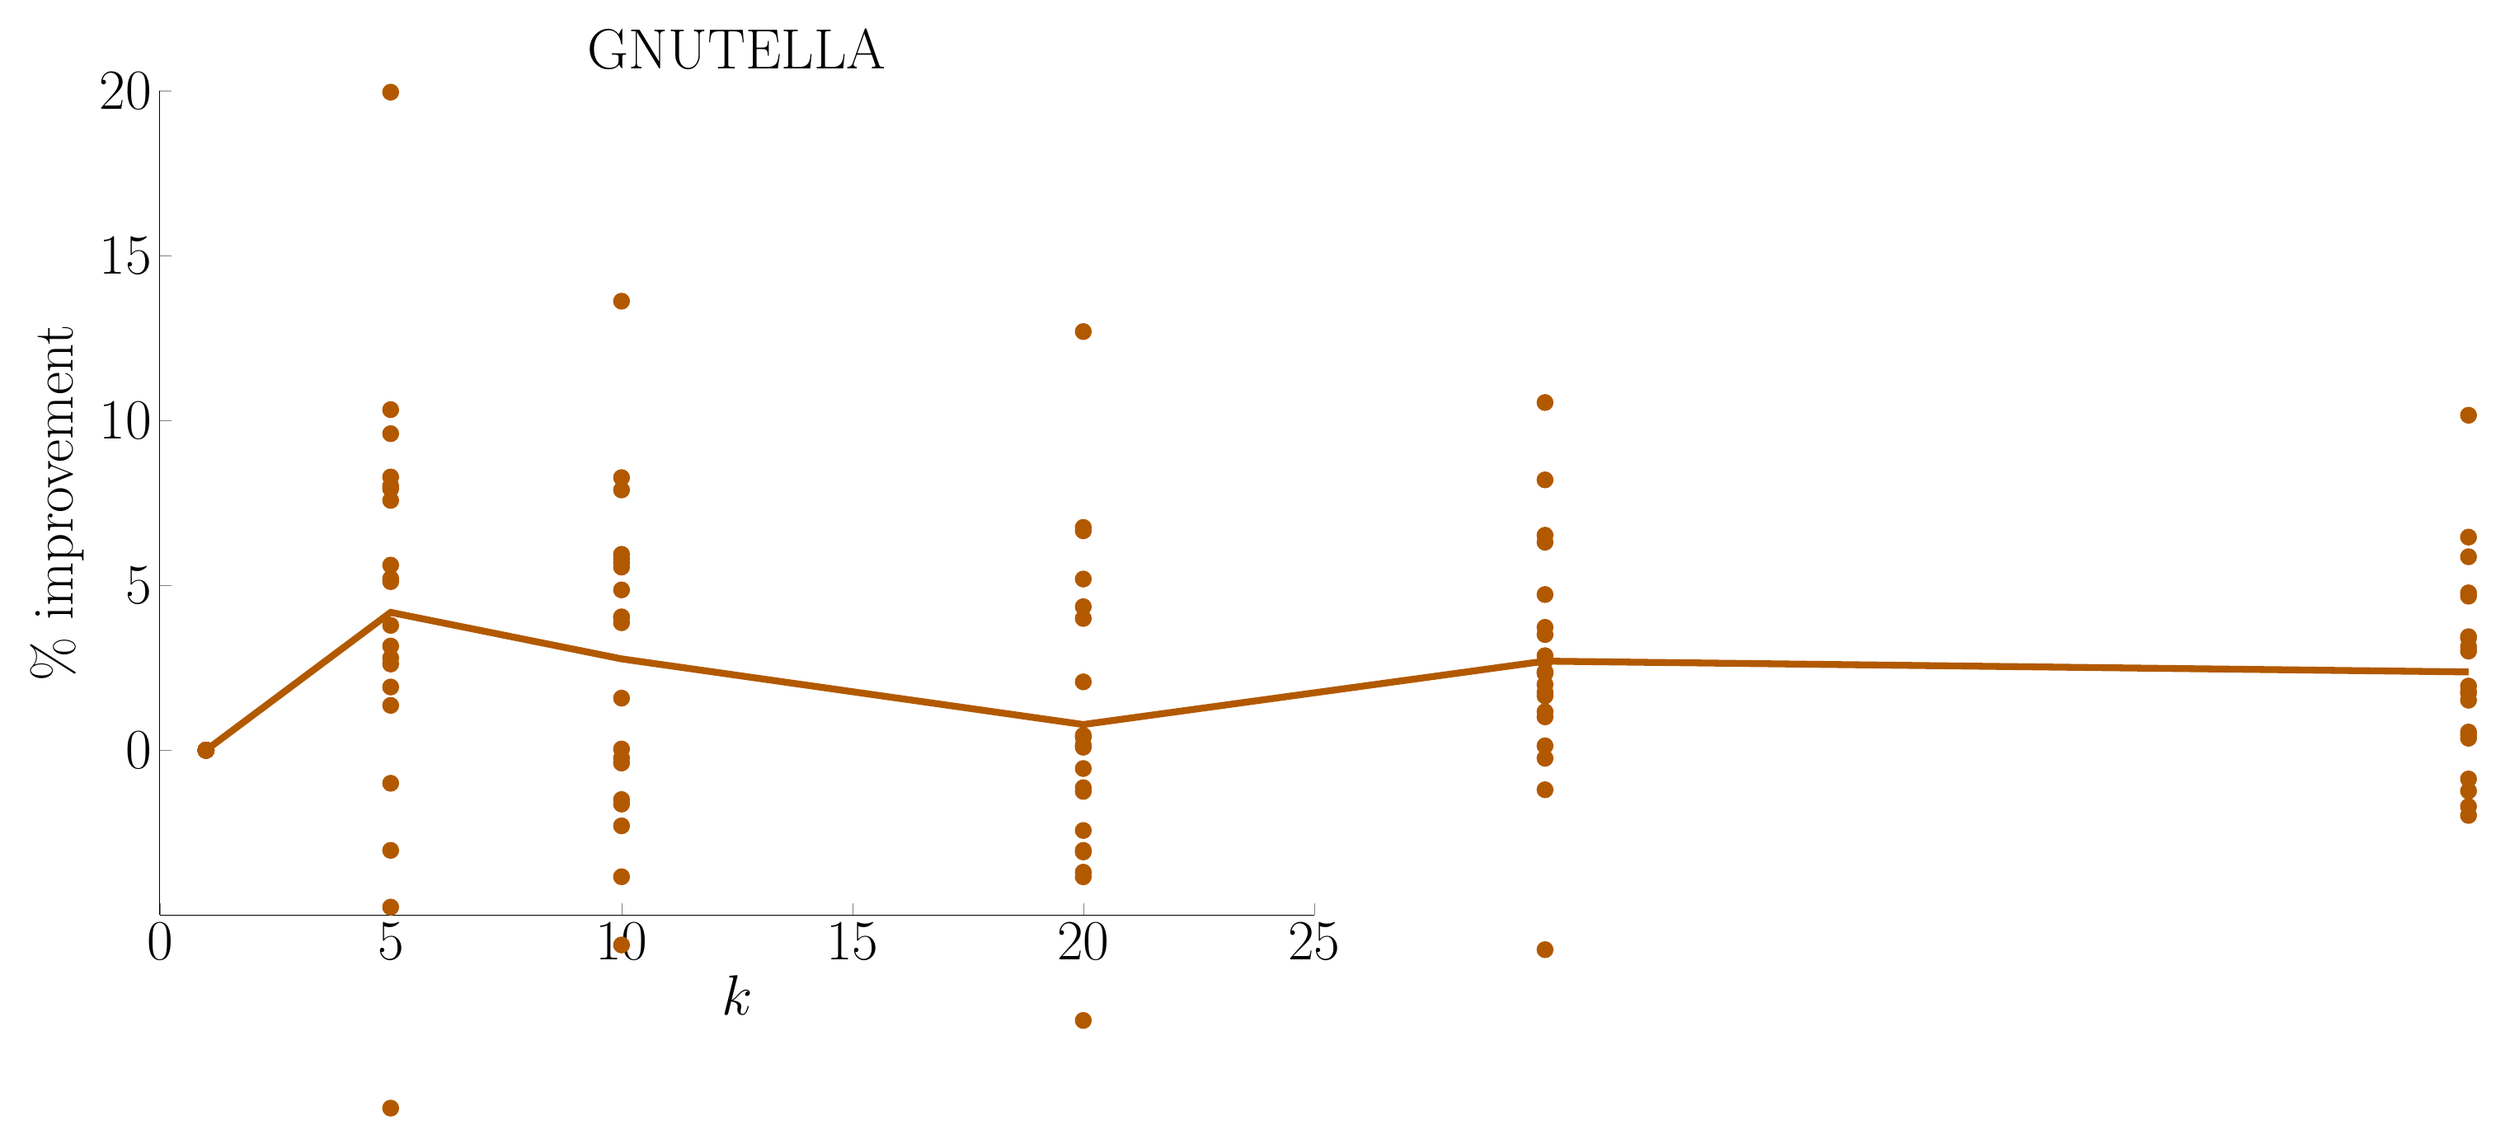
\begin{tikzpicture}

\begin{axis}[%
title style={font=\Huge},
title=GNUTELLA,
tick label style={font=\Huge},
label style={font=\Huge},
legend style={font=\Huge},
view={0}{90},
width=7in,
height=5in,
scale only axis,
xmin=0, xmax=25,
xtick={0, 5, 10, 15, 20, 25},
xlabel={$k$},
ymin=-5, ymax=20,
ytick={0, 5, 10, 15, 20},
ylabel={$\%$ improvement},
major tick length=5pt,
axis lines*=left,
legend cell align=left,
clip=false]

\addplot [
only marks,
mark=*,
mark size=3.5pt,
color=orange!70!black,
%solid,
%line width=2pt,
]
coordinates{
(1,0.0)(1,0.0)(1,0.0)(1,0.0)(1,0.0)(1,0.0)(1,0.0)(1,0.0)(1,0.0)(1,0.0)(1,0.0)(1,0.0)(1,0.0)(1,0.0)(1,0.0)(1,0.0)(1,0.0)(1,0.0)(1,0.0)(1,0.0)(5,-10.8558842039)(5,-4.75871313673)(5,-3.037184218)(5,-1.00143061516)(5,1.36)(5,1.91829484902)(5,2.6149968494)(5,2.80286515104)(5,3.16074653823)(5,3.78694581281)(5,5.11494252874)(5,5.208625035)(5,5.61474229773)(5,7.57820058046)(5,7.93092420851)(5,8.01589930441)(5,8.28854314003)(5,9.60274364104)(5,10.3322259136)(5,19.9616122841)(10,-5.90695243074)(10,-3.83751403969)(10,-2.29323308271)(10,-1.63321526958)(10,-1.49563772331)(10,-0.388838060384)(10,-0.239664469742)(10,0.0371195248701)(10,1.58045977011)(10,3.86769338467)(10,4.03031346883)(10,4.0465631929)(10,4.86356042324)(10,5.55555555556)(10,5.69967117282)(10,5.81109218247)(10,5.94310210444)(10,7.89574549636)(10,8.27009145748)(10,13.6214082036)(20,-8.19672131148)(20,-3.83936451898)(20,-3.69822485207)(20,-3.08527973927)(20,-3.03820428523)(20,-2.43381218093)(20,-1.24843945069)(20,-1.13607352566)(20,-0.554910311008)(20,0.0917536414726)(20,0.155242417005)(20,0.398502596305)(20,0.448811256672)(20,2.07424867413)(20,3.99798843349)(20,4.35451425867)(20,5.19313304721)(20,6.65665665666)(20,6.75881308648)(20,12.7001067236)(30,-6.04946000939)(30,-1.19893018537)(30,-0.243330146867)(30,0.134916351862)(30,1.01168672597)(30,1.16808382719)(30,1.64844851904)(30,1.75648021828)(30,1.99550794748)(30,2.33151504487)(30,2.37772353313)(30,2.71719038817)(30,2.86738351254)(30,3.50894340729)(30,3.72835004558)(30,4.72312703583)(30,6.30918073281)(30,6.52287718564)(30,8.20132569374)(30,10.5479019876)(50,-1.97740112994)(50,-1.70628459785)(50,-1.23589808594)(50,-0.871809578434)(50,0.364085560107)(50,0.459309095614)(50,0.552373158756)(50,1.51771800257)(50,1.74124449701)(50,1.76470588235)(50,1.94734699416)(50,3.00727670809)(50,3.14250756649)(50,3.40925066779)(50,3.44401041667)(50,4.67308598748)(50,4.77476869048)(50,5.86884775434)(50,6.46502293578)(50,10.1614035088)
};

\addplot [
color=orange!70!black,
solid,
line width=3pt
]
coordinates{
(1,0.0)(5,4.18195479802)(10,2.77136604306)(20,0.779937030819)(30,2.70294609077)(50,2.37507820172)
};

\end{axis}
\end{tikzpicture}
\end{document}
